% Beskriv hvilke valg der ligger til grund for designet af vores model
% hvad lægger vi vægt på? 
% Koncentet med en drone, en slave og en master - skalérbarhed
% Brugere, rettigheder, permissions osv.


\section{Idea}
We want an architecture that supports three things:

\begin{itemize}
	\item Drone and User interaction
	\item Different access to the system on a per user basis 
	\item Scalability in regard to both usage and the scope of the system
\end{itemize}

These architectural goals are a mixture of the requirements of this project and the needs described in the analysis. 
They will be described in the following. 


\subsection{Drone and User interaction}
A User should be able to interact with a Drone via the system.
This includes both watching the video feed and controlling the Drones movements.
This is one of the most important features in the system.
Therefore it is important the the systems architecture supports it natively. 


\subsection{Different access to the system on a per user basis}
Another important feature is support of multiple users and drones, and not least support of different access level for different users.
Not all users should be able to see all drones, and therefore some security/access system needs to be implemented into the model. 


\subsection{Scalability in regard to both usage and the scope of the system}
The security/access system makes sure that the system is scalable in regard to adding more users or drones. 
But the architecture must also make sure that the system does not only scale up, but also out. 
There may come a point where the system needs to support other objects than drones, such as stationary cameras or other equipment. 
In that situation the system needs to be able to handle this without needing to change the source code first.
Therefore, this must be a part of the architecture already now. 


\subsection{Communication between a Drone and the web service}
Since the AR Drones are broadcasting their own WIFI network that one can connect to, instead of being able to connect to an existing WIFI network, them implementation is sort of backwards. 
This means that the Drone is not able to connect directly to the web service. 

\begin{figure}[htb]
    \centering
    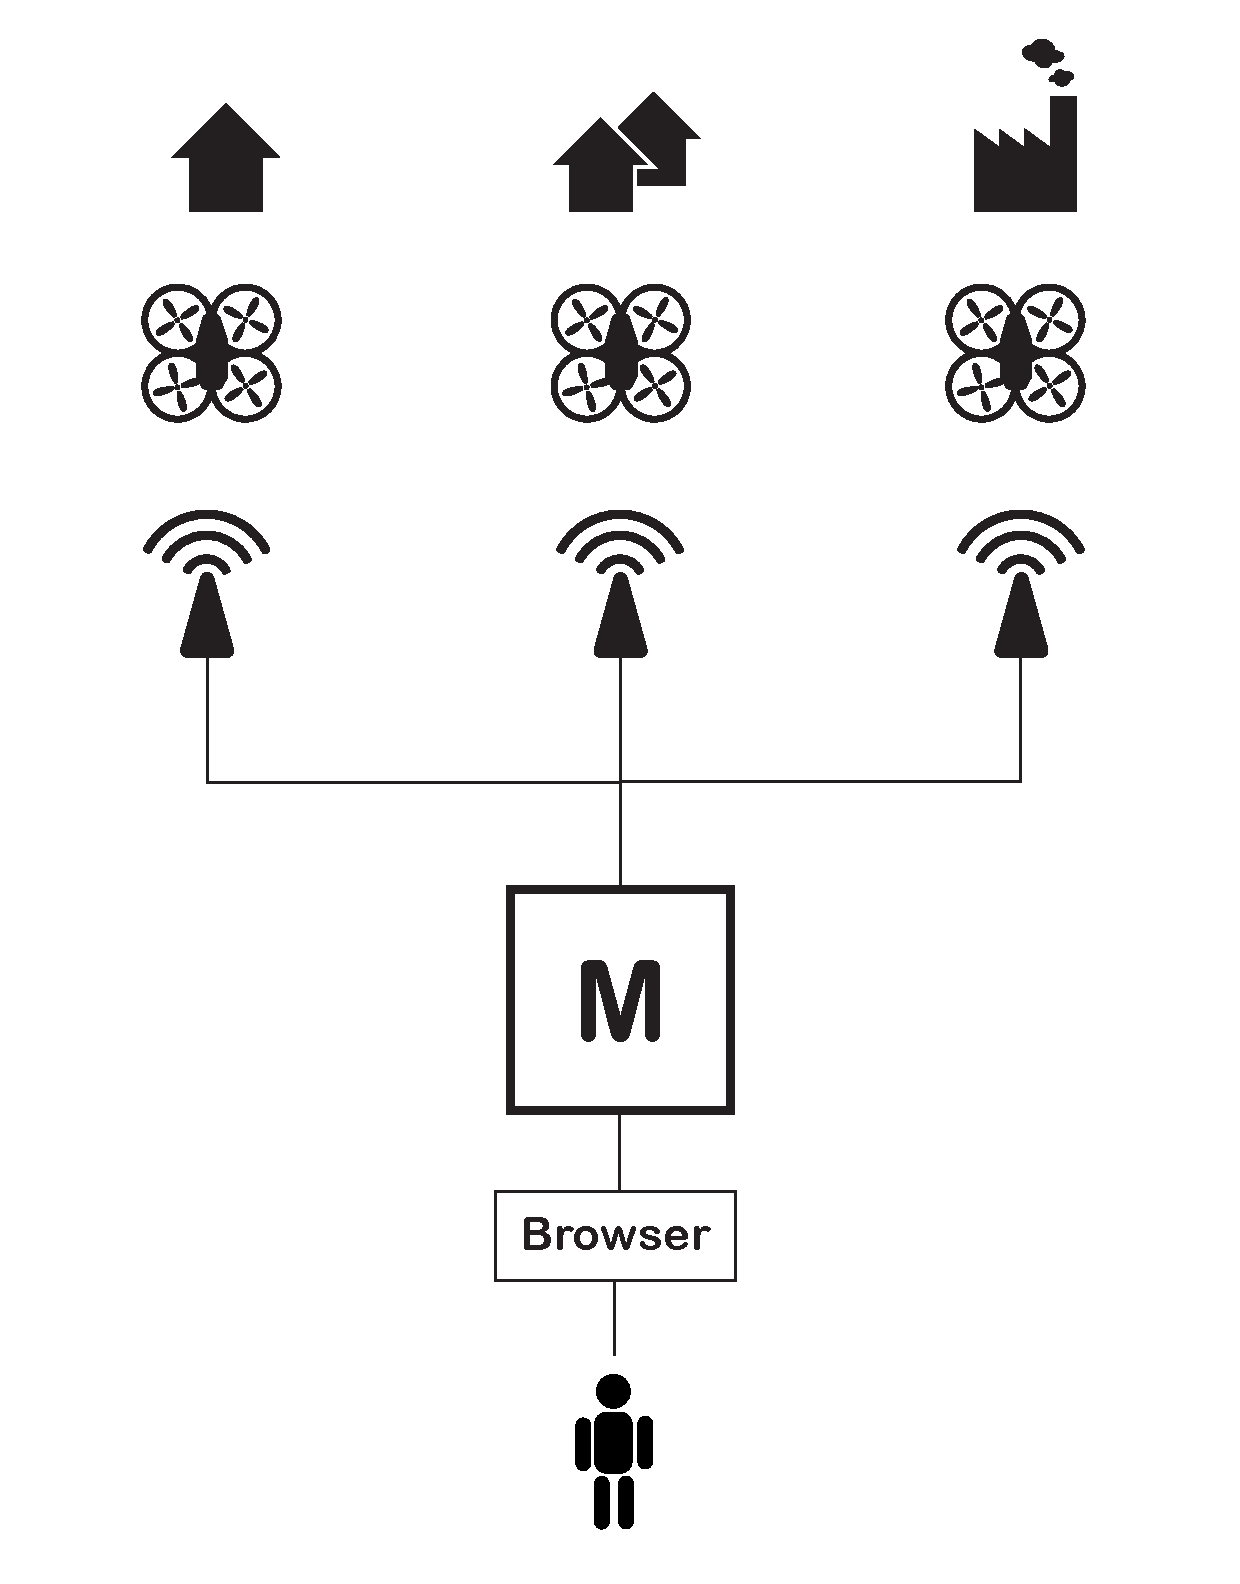
\includegraphics[width=\textwidth]{gfx/technical_structure.pdf}
    \caption{Illustration of the relationship between Drones and the end User}
    \label{fig:Technical_Structure}
\end{figure}

Figure~\ref{fig:Technical_Structure} shows the architecture of the physical elements (drones, servers and users) and is also an example with one user and three drones, each located at three different locations.
Due to the AR Drones nature where they broadcast a WIFI that a client must connect to, each location has a ``Slave''-server that connects to a Drones WIFI. 
Each client then communicates with the ``Master''-server (which is also hosting the web service), which a user can connect to via his Internet Browser. 
That means that the communications flow from the user to the drone will be as displayed in Figure~\ref{fig:Technical_Structure}.
